
\chapter{Appendix: Guided Stable Dynamic Projections}

\section{PCD-tSNE parameters}

Table \ref{tab:pcd-params} presents the PCD-tSNE parameters used for each dataset. This table compliments Sec. 3.2 of the main text. 

\begin{table}[h!]
  \centering
  \fontfamily{lmss}\selectfont
  \scriptsize
  %\setlength\tabcolsep{2pt} % default value: 6pt
  %\scriptsize
  %\centering
  \begin{tabular}{|l|l|l|}
  \hline
 % \multicolumn{3}{|c|}{PCD-tSNE parameters} \\
 % \hline
  {dataset}    & {$\lambda$} & {PC scaling}        \\ \hline
  \hline
  cartolastd & $10^{-2}$ & $10^{0}$  \\ \hline
  cifar10cnn & $10^{-5}$ & $10^{0}$  \\ \hline
  esc50      & $10^{-2}$ & $10^{-1}$ \\ \hline
  fashion    & $10^{-4}$ & $10^{-1}$ \\ \hline
  gaussians  & $10^{-3}$ & $10^{1}$  \\ \hline
  nnset      & $10^{-3}$ & $10^{0}$  \\ \hline
  qtables    & $10^{-3}$ & $10^{-1}$ \\ \hline
  quickdraw  & $10^{-3}$ & $10^{0}$  \\ \hline
  sorts      & $10^{-1}$ & $10^{0}$  \\ \hline
  walk       & $10^{-4}$ & $10^{0}$  \\ \hline
  \end{tabular}
  \caption{The $\lambda$ parameter modulates the amount of global influence applied to points in $P(\mathbf{D}^t)$; the \emph{PC scaling} term scales $W$ to increase/decrease the area of global influence, i.e., it scales the principal components of \,$\mathbf{D}$.}
  \label{tab:pcd-params}
\end{table}

\section{LD-tSNE parameters}

Table \ref{tab:ld-params} presents the LD-tSNE parameters used for each dataset. This table compliments Sec. 3.1 and Sec. 5.5 of the main text. 

\begin{table}[ht!]
  \centering
  \fontfamily{lmss}\selectfont
  \scriptsize
  %\setlength\tabcolsep{2pt} % default value: 6pt
  %\scriptsize
  %\centering
  \begin{tabular}{|l|l|l|l|l|}
    \hline
%    \multicolumn{5}{|c|}{LD-tSNE parameters} \\
%    \hline
  dataset    & $\lambda$ & $\beta$ & $\alpha$ & $\mathbf{l}^q$ projection (\# landmarks) \\ \hline
  \hline
  cartolastd & .2     & 2  & 4  & PCA($N$)                 \\ \hline
  cifar10cnn & .5     & 4  & 1  & tSNE($N$)               \\ \hline
  esc50      & .3     & 5  & 1  & PCA($N$)                 \\ \hline
  fashion    & .1     & 4  & 2  & tSNE($N$)               \\ \hline
  gaussians  & -      & -  & -  & PCA($N$)                 \\ \hline
  nnset      & .02    & 8  & 1  & PCA($N$)                 \\ \hline
  qtables    & -      & -  & -  & PCA($N$)                 \\ \hline
  quickdraw  & .1     & 2  & 1  & tSNE($N$)               \\ \hline
  sorts      & .25    & 10 & 2  & PCA($NT$)               \\ \hline
  walk       & -      & -  & -  & PCA($N$)                 \\ \hline
  \end{tabular}
  \caption{The $\lambda$, $\alpha$, and $\beta$ parameters control the amount of influence landmarks have on the the points being projected. In simple terms, $\alpha$ controls the tightness of clusters in $P(\mathbf{D}^t)$, $\beta$ scales the strength of the ``pull'' of landmarks $\mathbf{L}$ on points in $P(\mathbf{D}^t)$, and $\lambda$ balances the two factors. 
  Values marked ``-'' were obtained using the interactive mode that was implemented and gave the user real-time control over parameters during the optimization. $N$ is the number of points in $\mathbf{D}^t$ and $T$ is the total number of timesteps in $\mathbf{D}$.}
  \label{tab:ld-params}
\end{table}


\section{Metric results}

Table \ref{tab:unaggregated} shows unaggregated metric results. Each of the 10 subtables correspond to a dataset, columns correspond to the different quality metrics, and the rows represent the different methods.
Methods are ordered according to their strategy: Per-timeframe, Global, Continuous, and Guided. 
The columns correspond, respectively, to distance preservation metrics ($S_{Pearson}, S_{Spearman}, S_{Kendall}, S_{Stress}$), neighborhood preservation metrics ($S_{NH}, S_{NP}, S_{Trust}, S_{Cont}$), and temporal stability metrics ()$T_{Pearson}, T_{Spearman}, T_{Kendall}, T_{Stress}$). The colormap is normalized independently for each metric and each dataset.

These tables compliment Sections 5.2 and 5.3 of the main text.


\begin{table}[h]
\begin{tabular}{c}
  \vspace{-.1cm}
  
\includegraphics[width=\linewidth]{figures/projection-algorithm/table_header.png} \\
  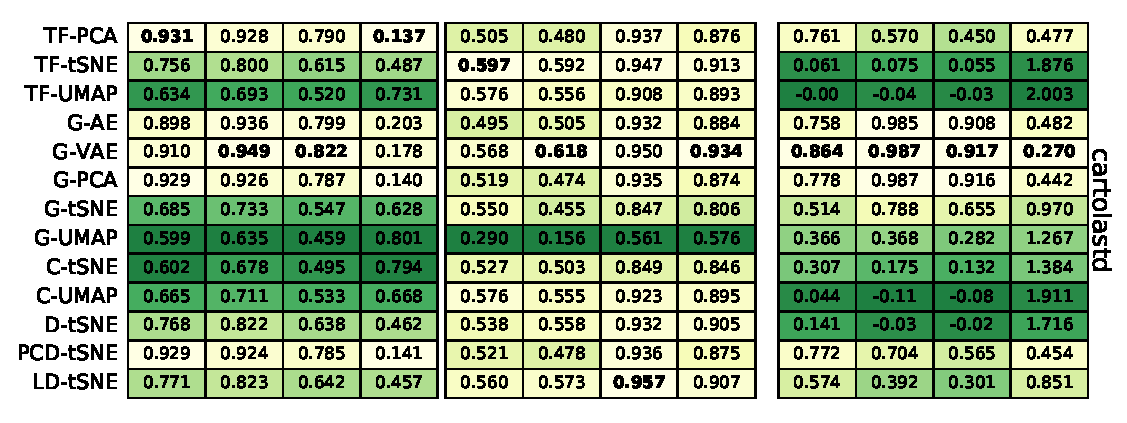
\includegraphics[width=\linewidth]{figures/projection-algorithm/table_cartolastd.eps} \\
  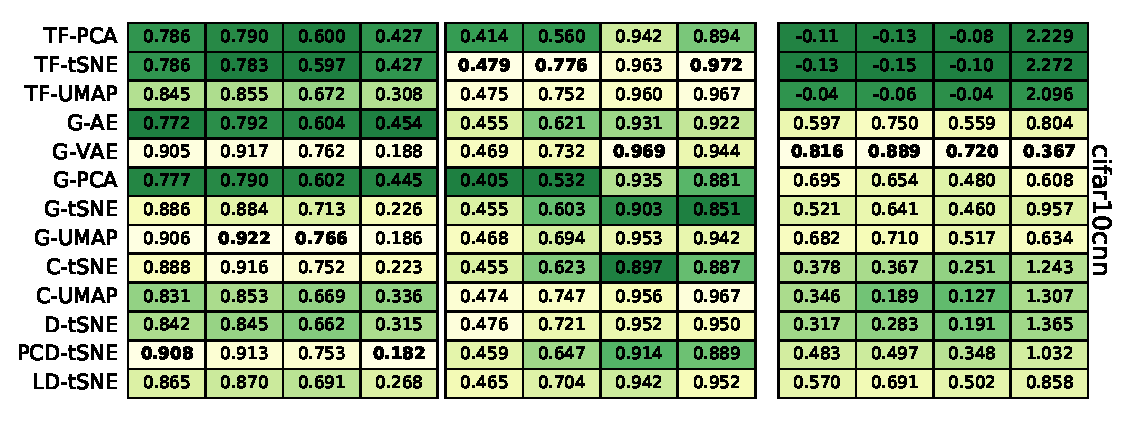
\includegraphics[width=\linewidth]{figures/projection-algorithm/table_cifar10cnn.eps} \\ 
  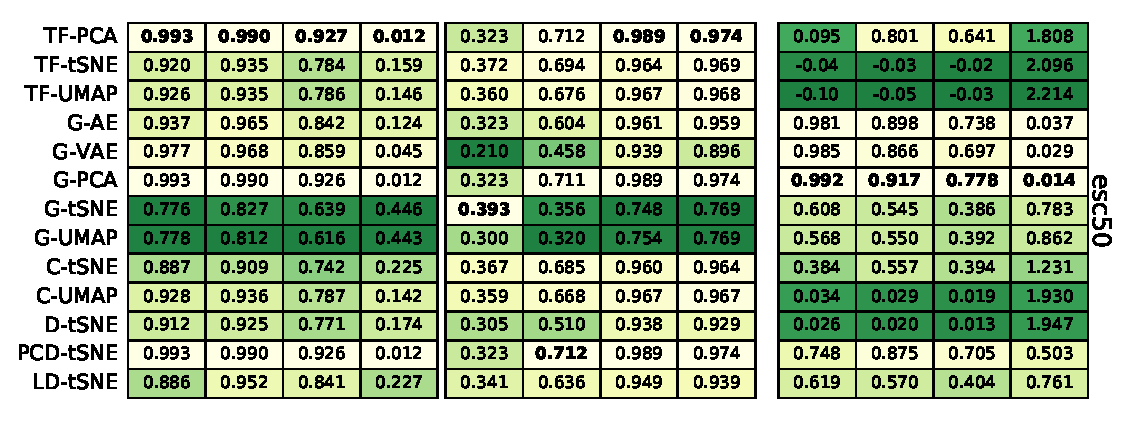
\includegraphics[width=\linewidth]{figures/projection-algorithm/table_esc50.eps} \\
  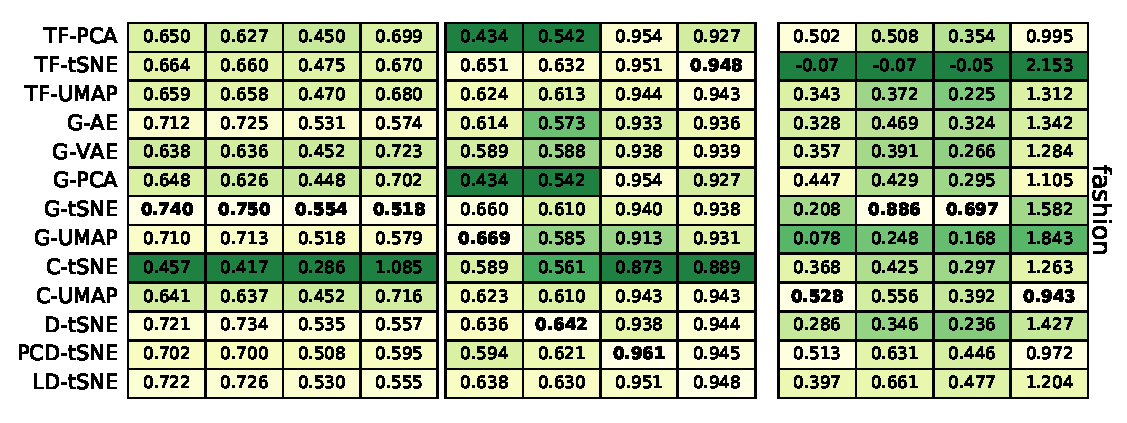
\includegraphics[width=\linewidth]{figures/projection-algorithm/table_fashion.eps} \\
\end{tabular}
\end{table}


\begin{table}[h]
\begin{tabular}{c}
    \vspace{-.1cm}
    
\includegraphics[width=\linewidth]{figures/projection-algorithm/table_header.png} \\
    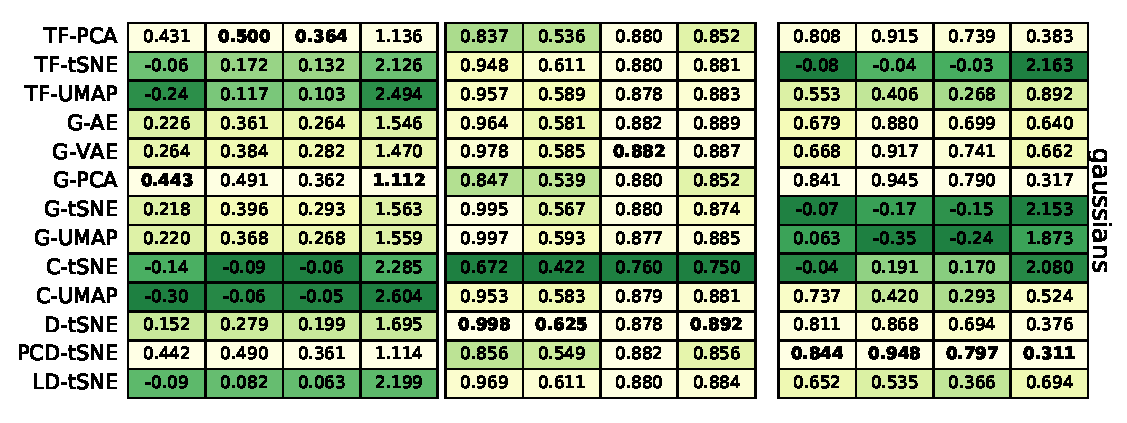
\includegraphics[width=\linewidth]{figures/projection-algorithm/table_gaussians.eps} \\
    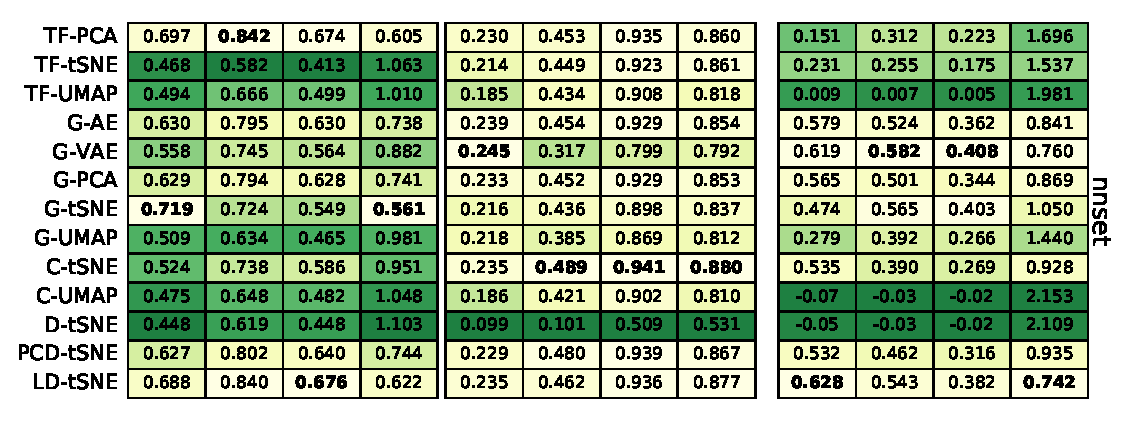
\includegraphics[width=\linewidth]{figures/projection-algorithm/table_nnset.eps} \\
    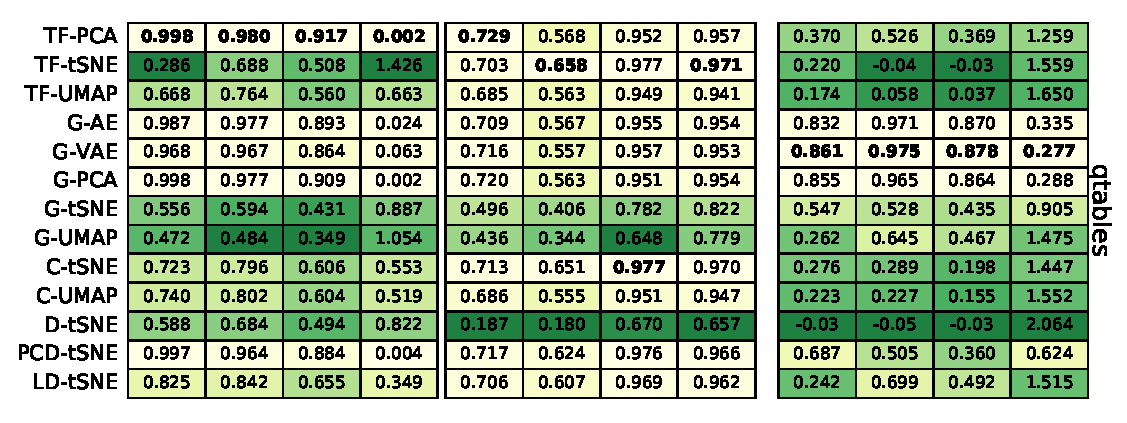
\includegraphics[width=\linewidth]{figures/projection-algorithm/table_qtables.eps} \\
    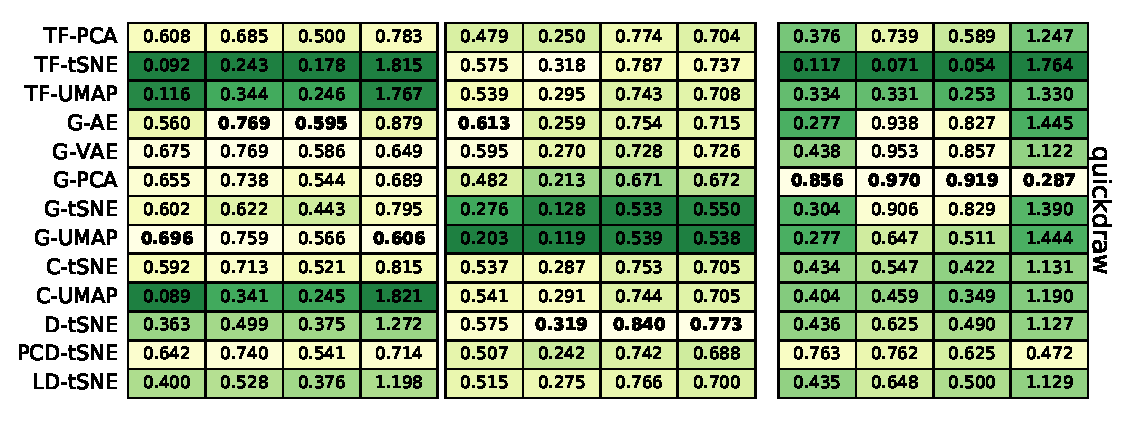
\includegraphics[width=\linewidth]{figures/projection-algorithm/table_quickdraw.eps} \\
    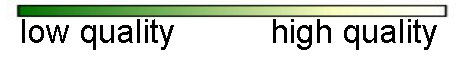
\includegraphics[width=.35\linewidth]{figures/projection-algorithm/green-colormap.pdf} \\
\end{tabular}
\end{table}
    

\begin{table}[h]
\begin{tabular}{c}
  \vspace{-.1cm}
  
\includegraphics[width=\linewidth]{figures/projection-algorithm/table_header.png} \\
  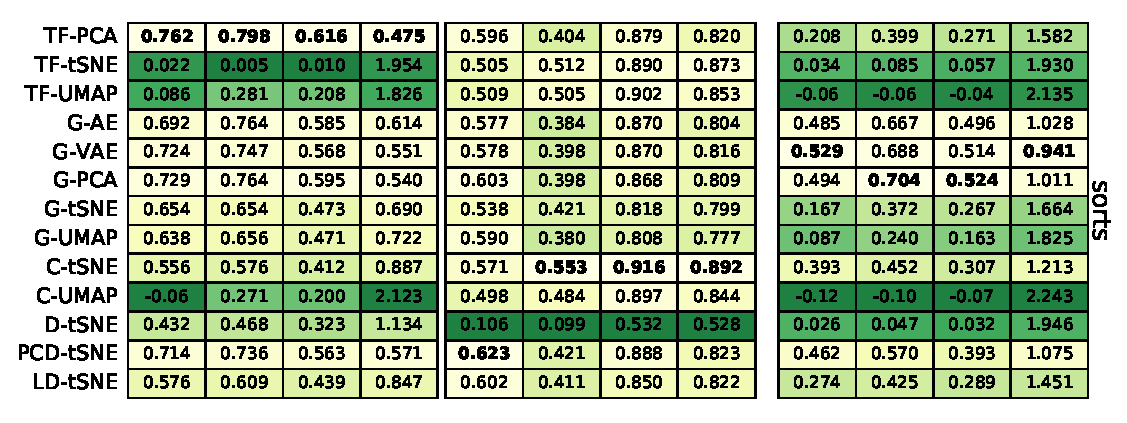
\includegraphics[width=\linewidth]{figures/projection-algorithm/table_sorts.eps} \\
  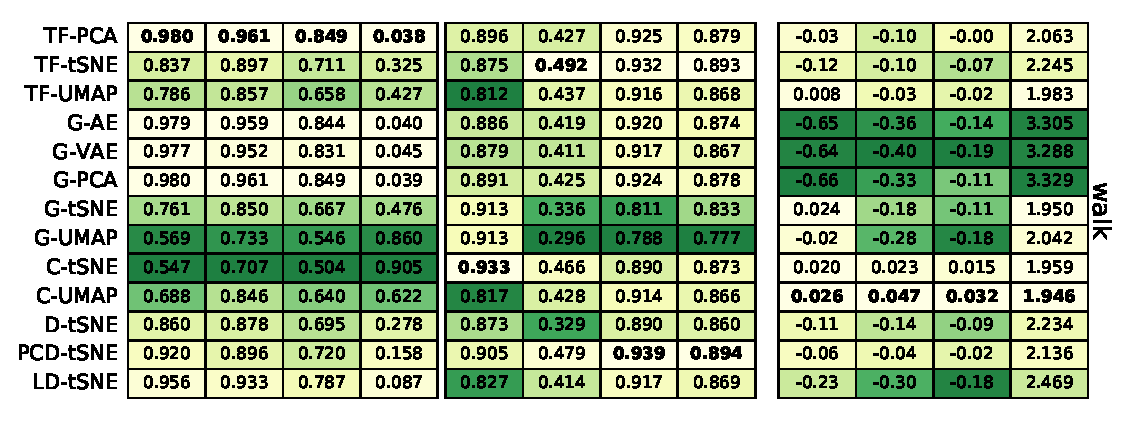
\includegraphics[width=\linewidth]{figures/projection-algorithm/table_walk.eps} \\
  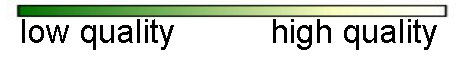
\includegraphics[width=.35\linewidth]{figures/projection-algorithm/green-colormap.pdf} \\
\end{tabular}
\caption{Unaggregated metric results.}
\label{tab:unaggregated}
\end{table}


%  \red{ld-tsne - the (-) are placed in runs that I chose the values in "interactive" mode and didn't write the final hyperparameters down. Beta is global exageration, and alpha is local exageration, as seen in formula. Projection (\# points) refers to the projection method used to project the landmarks and the number of landmarks. -}}



% HALF PAGE WIDTH FIGURE
% \begin{figure}[tb]\centering
%   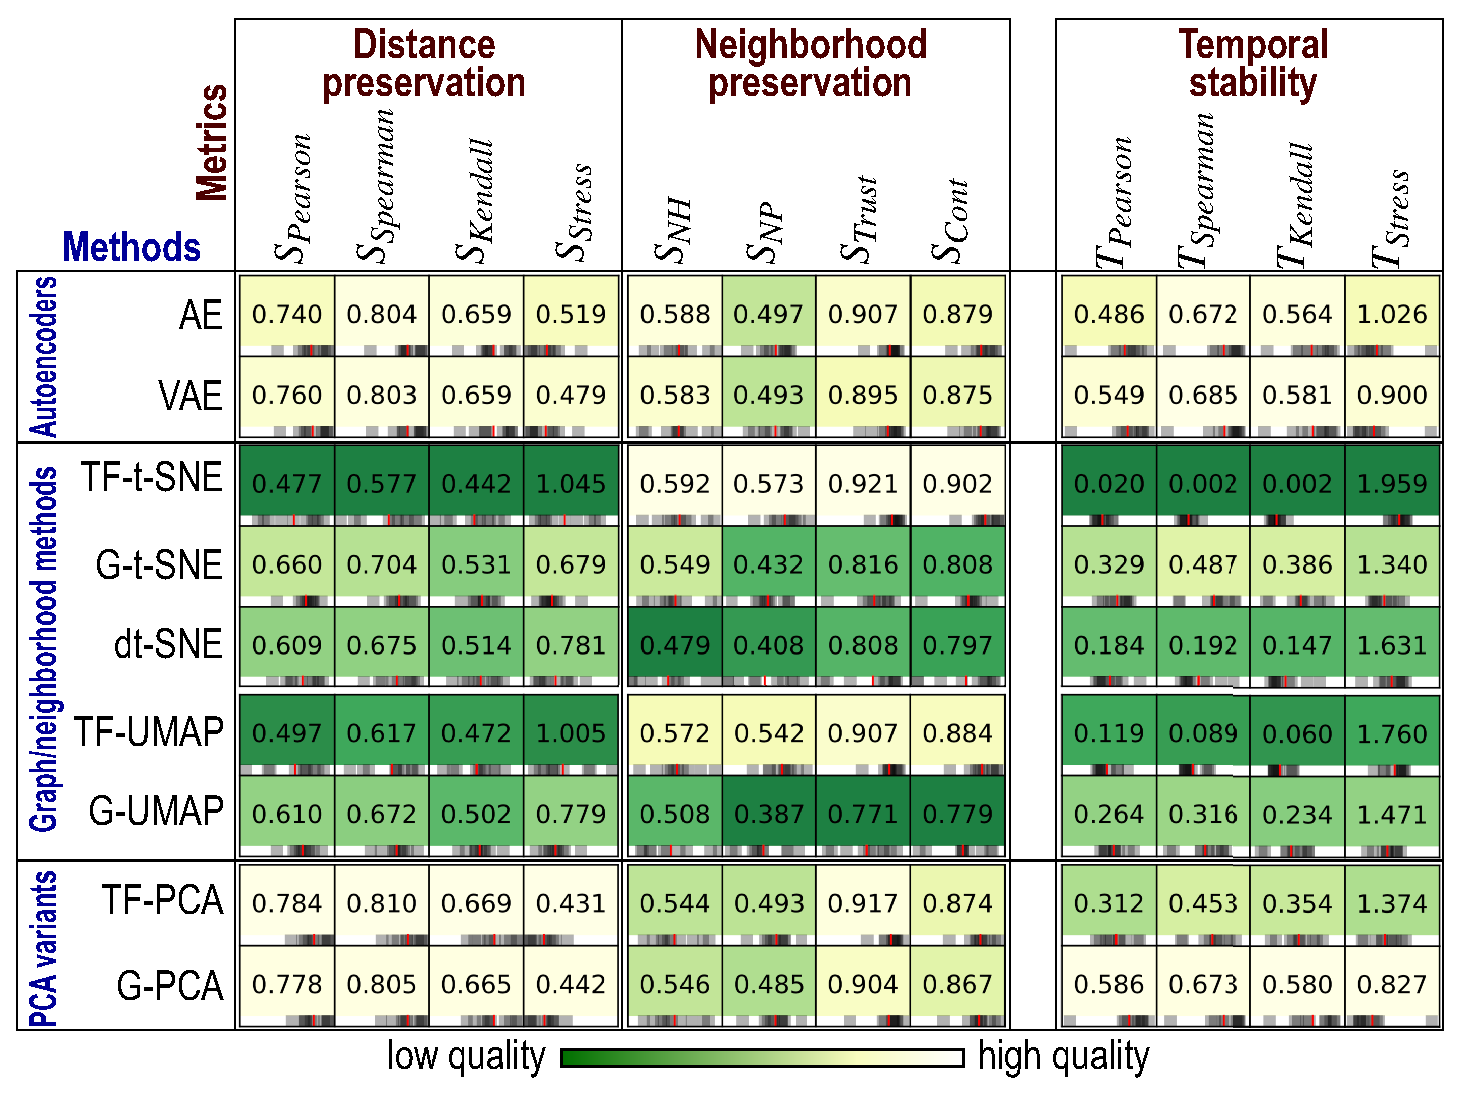
\includegraphics[width=.95\linewidth]{images/aggregate_matrix.eps}
%   \caption{Aggregated metric results over all datasets.}
%   \label{fig:aggregated}
% \end{figure}

% FULL PAGE WIDTH FIGURE
% \begin{figure*}[!tb]
%   \centering
%   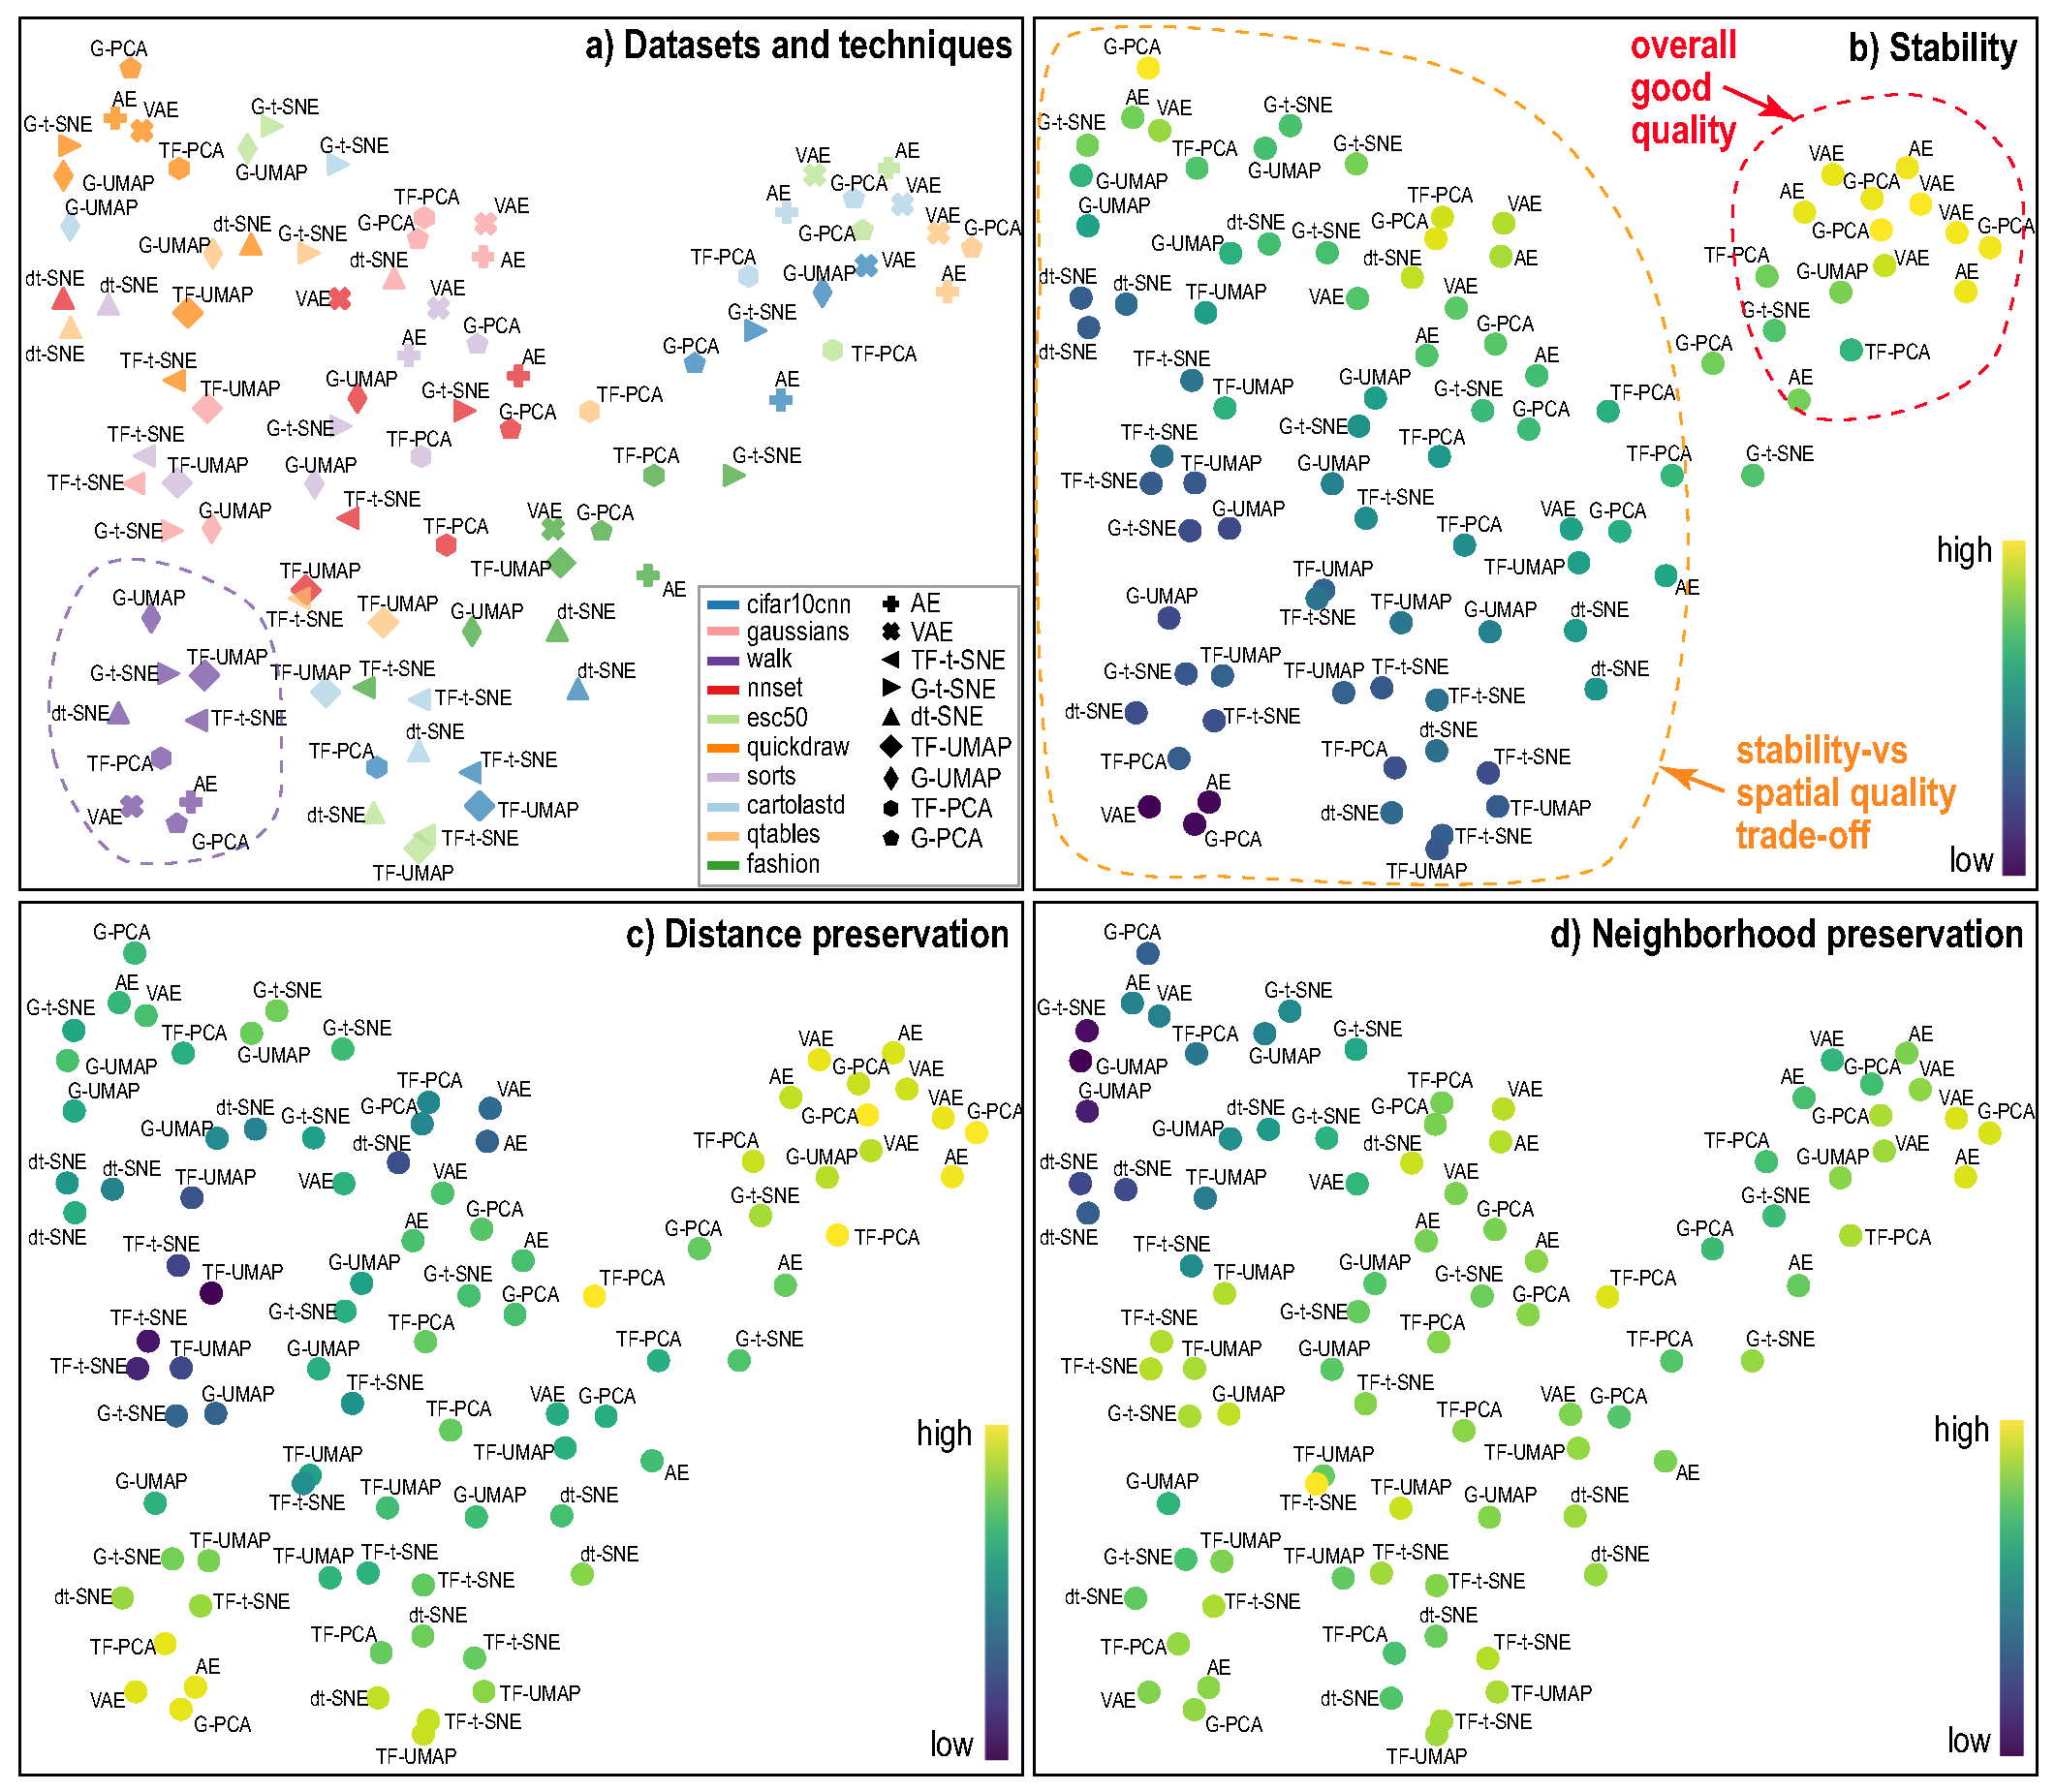
\includegraphics[width=0.7\linewidth]{images/summary_plots.eps}
%   \caption{Projection of projections map showing the similarity of all evaluated techniques on all datasets (Sec.~\ref{sec:choice}).}
%   \label{fig:tsne_0}
%   \end{figure*}


%-------------------------------------------------------------------------
